\section{SISTEMA DE SOFTWARE DO FUTEBOL DE ROBÔS}

O sistema deste time pode ser representado simplificadamente através do diagrama apresentado na Fig. \ref{fig:esquema_software} que indica as partes principais do processamento. Estas partes são descritas, juntamente com as interações entre elas, na sequência. A CÂMERA captura uma imagem do campo, esta imagem é então processada pelo módulo de VISÃO que determinará as posições atuais dos robôs a partir de suas etiquetas coloridas e a da bola que possui cor alaranjada. A PREVISÃO, com base das informações recebidas do módulo da VISÃO, define as posições mais prováveis que os objetos em campo irão assumir alguns instantes a frente. Com estas posições (presente e futura). O módulo de ESTRATÉGIA calcula os locais do campo que os robôs do time controlado deverão se posicionar. Para realizar estes cálculos, este módulo faz uso de roteiros, que são específicos para cada robô. Basicamente, um roteiro é um conjunto de comportamentos específicos para cara robô que faz com que este assuma uma postura defensiva ou ofenciva durante uma partida. O módulo de CONTROLE, fazendo uso das posição atuais de cada robô (VISÃO) e de seus objetivos (ESTRATÉGIA), determina maior velocidade possível que um robô pode assumir para que este consiga chegar ao seu objetivo e parar, definindo os valores de cada roda a serem enviados aos robôs via rádio, fazendo os robôs se moverem para concluir a estratégia. Todos estes módulos são executados no computador pessoal.

% FIGURA
\begin{figure}[!htb]
  \centering
  % 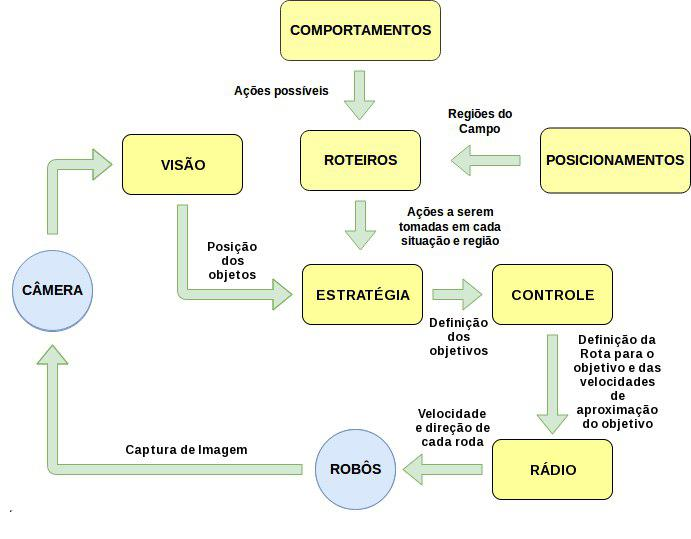
\includegraphics[width=240pt, height=190pt]{esquema_software.jpg}
  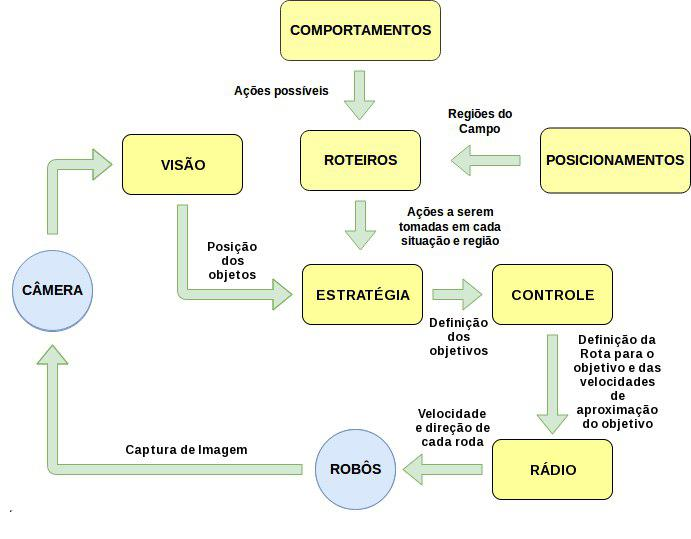
\includegraphics[scale=0.35]{esquema_software.jpg}
  \caption{Diagrama simplificado dos módulos do time Carrossel Caipira.}
  \label{fig:esquema_software}
\end{figure}
%%%

\subsection{Módulo da Visão}

No ambiente de futebol de robôs toda a estratégia e o controle, tanto de baixo nível quanto de alto nível, são baseados na interpretação das imagens captadas pela câmera. Para que isso seja realizado, etiquetas de cores em destaque localizadas no topo dos robôs identificam cada um deles, em relação a seu time e possivelmente sua função, conforme demonstra a Fig. \ref{fig:etiqueta}.

O tempo de execução do ciclo de controle do sistema foi definido pela taxa de aquisição de imagens. Como o time Carrossel Caipira usa câmeras de vídeo convencionais, a taxa é limitada a 30 quadros por segundo. Portanto, a cada período de 33 ms, uma nova imagem refletindo o estado atual do campo torna-se disponível ao computador para processamento. Cada uma dessas imagens é capturada e digitalizada por uma placa
de captura, que disponibiliza, na forma de uma matriz com dimensões 640x480 pixels com três canais (componentes Red, Green, Blue - RGB). Cada um desses pixels deve ser analisado, quanto a sua cor, para identificar se é uma cor de importância ao sistema, esta técnica é chamada de segmentação de cor.

% FIGURA
\begin{figure}[!htb]
\centering
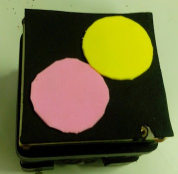
\includegraphics[scale=0.9]{etiqueta.png}
\caption{ Etiqueta de identificação do robô}
\label{fig:etiqueta}
\end{figure}
%%%

\subsection{Módulo de Estratégia}

A estratégia é o módulo responsável por definir a meta de cada robô. Utilizando as coordenadas da bola, dos robôs do time e dos adversários este módulo decide qual é a posição mais indicada para cada robô do time através dos roteiros. Os roteiros são basicamente conjuntos de regras que ditam o comportamento do robô em cada situação. Com as posições pré-determinadas no módulo de posicionamentos e com os comportamentos padronizados no módulo de comportamentos, os roteiros são montados pensando nas situações de jogo. A vantagem deste modelo em relação aos antigos é que através da padronização dos elementos mais básicos da estratégia através destes dois novos módulos é possível montar facilmente montar novos roteiros, o que permite que o time possua diversas posturas às mais diversas situações de jogo, sendo mais ofensivo quando estiver atrás no placar ou mais defensivo quando se deseja tentar manter o resultado, por exemplo.

\subsection{Módulo de Controle}

A partir das coordenadas detectadas pelo módulo de Visão e das coordenadas atribuídas pelos resultados do módulo de Estratégia, o módulo de Controle deve determinar as melhores trajetórias e comandos a ser enviados aos robôs. O cálculo de uma trajetória deve levar em conta o desvio de obstáculos, evitando os outros robôs na arena. Este cálculo é necessário para levar o robô da sua posição atual até a determinada pela estratégia. No caso do time Carrossel Caipira, é empregado um método chamado de campo potencial. Os campos potenciais partem da ideia de forças imaginárias atuando sobre o robô, ideia proposta por Khatib [4], na qual a ''força causada'' pelos obstáculos é de caráter repulsivo e pela meta, de caráter atrativo. Porém a interferência das ''forças'' geradas a partir de vários obstáculos podem produzir locais
ótimos que atrapalham o desempenho do sistema para encontrar um caminho até a meta para o robô.

Para evitar esta situação, Connoly et al. [5] solucionaram o problema utilizando funções harmônicas para o cálculo do campo potencial de ambientes nos quais as posições das paredes, objetos e metas sejam conhecidas, que é o caso do ambiente de futebol de robôs. As funções harmônicas utilizadas são soluções para a equação de Laplace (1).
%
\begin{equation}
\nabla = 0 \ para \ P : R \rightarrow R .
\end{equation}

Assim é definido um Problema de Valor de Contorno na região de atuação do robô utilizando a condição de Dirichlet%
%
\footnote{A condição de contorno de Dirichlet (ou de primeiro tipo) é um tipo de condição de contorno, nomeada em homenagem a Johann Peter Gustav Lejeune Dirichlet (1805-1859). Quando aplicada sobre uma equação diferencial ordinária ou parcial, especifica os valores que uma solução necessita para tomar-se sobre o contorno do domínio}
%
com potencial alto para obstáculos e potencial baixo para a meta. Então, são extraídas as linhas de força, com base no gradiente descendente [5][6] do potencial, que direcionam o robô para sua meta, desviando-o de obstáculos.

Uma vez obtido o campo potencial, tem-se o ângulo ideal que o robô deve atingir para se deslocar até a meta, que chamamos de ângulo objetivo, basta agora calcular a direção e velocidade de cada motor.

\subsection{Interface}

Para comportar toda essas mudanças feitas em diversos módulos da equipe foi também desenvolvida uma nova interface, tendo em mente praticidade e as necessidades de comportar novas funcionalidades. A nova interface foi feita utilizando abas para as principais seções, entre a principal, configurações, outros e ajuda, como pode ser observado na Fig. \ref{fig:interface}.

Na aba principal o foco foi deixar de fácil acesso as funções indispensáveis durante o jogo, entre uma tela para mostrar o q está sendo captado pela câmera, uma tabela para logs e botões para iniciar o software além de situação em que o jogo está, como jogo normal, disputa de bola, w.o., entre outros.

Na aba de configurações se encontram as principais configurações indispensáveis para setup do software, entre escolha dos roteiros, calibração da visão entre outras.

Na aba outros, foram colocadas configurações que geralmente não são usadas, porém podem vir a ser necessárias em situações inesperadas, entre uma opção para gravação em buffer de alguns frames de jogo, uma opção para capturar uma imagem do campo vazio, entre outras.

Finalmente a aba ajuda tem por finalidade explicar as mais diversas funcionalidades do programa, através de uma estrutura separada em seções, pessoas que não conhecem o software podem aprender sobre como utilizá-lo.

% FIGURA
\begin{figure}[!htb]
\centering
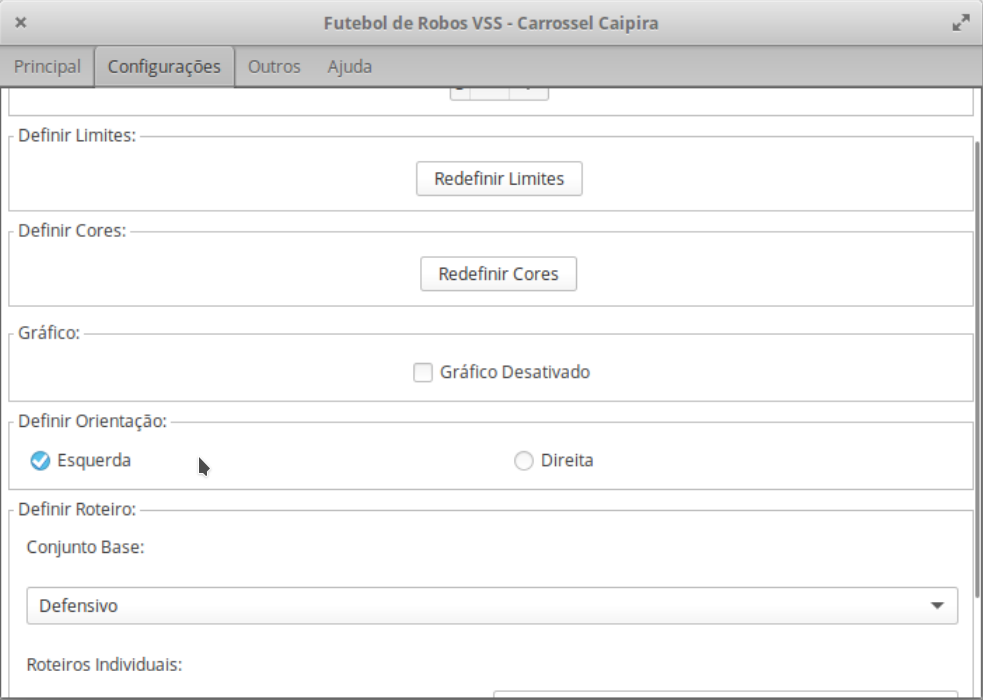
\includegraphics[scale=0.3]{interface.png}
\caption{Nova interface na aba de configurações.}
\label{fig:interface}
\end{figure}
%%%
